\documentclass{beamer}
\usepackage[UTF8]{ctex}

\usetheme{metropolis}
\setbeamerfont{title}{size=\zihao 4}
\usepackage{appendixnumberbeamer}
\usepackage{amsmath}
\usepackage{enumerate}
\usepackage{tabu}
\usepackage{multirow}
\usepackage{makecell}
\usepackage{tikz}
\usepackage{amsmath}
\usepackage{algorithm}
\usepackage{algorithmic}
\usetikzlibrary{matrix,calc,shapes,backgrounds,patterns,positioning,decorations.pathreplacing}

\floatname{algorithm}{算法}
%\newcommand\forthsection[1]{\noindent \S #1}
\renewcommand{\algorithmicrequire}{ \textbf{输入:}} %Use Input in the format of Algorithm  
\renewcommand{\algorithmicensure}{ \textbf{输出:}} %UseOutput in the format of Algorithm
% \renewcommand\theequation{\arabic{chapter}-\arabic{equation}}
\renewcommand{\thealgorithm}{}

\title{基于Spatial-Spark网络空间海量数据分析与挖掘}
\author[高峰]{
    \makebox[2.5em][s]{姓名:} \makebox[3em][s]{高峰}\\
    \makebox[2.5em][s]{导师:} \makebox[3em][s]{高井祥} \\
    \makebox[2.5em][s]{} \makebox[3em]{孙久运} \\
    \makebox[2.5em][s]{专业:} \makebox[10em][l]{大地测量学与测量工程}\\
}
\date{}
\titlegraphic{\hfill
\includegraphics[height=1.5cm]{figures/cumt.pdf}}

\begin{document}
% make title
\maketitle

% make content
\begin{frame}{提纲}
  \setbeamertemplate{section in toc}[sections numbered]
  \tableofcontents[hideallsubsections]
\end{frame}

% \section{绪论}

% \begin{frame}{绪论}
%     \begin{columns}
%         \begin{column}{0.5\textwidth}
%         \includegraphics[scale=0.3]{figures/smartcity.jpg}
%         \end{column}

%         \begin{column}{0.5\textwidth}
%         \textbf{智慧城市:} 
        
%         数字城市、物联网、云计算
%         % \includegraphics[scale=0.2]{figures/smartcity.jpg}
%         \vspace{2em}

%         \pause
%         \alert{数字城市}
%         \begin{itemize}
%         \pause
%         \item 空间信息快速获取技术
%         \pause
%         \item 海量空间数据管理
%         \pause
%         \item 空间信息可视化技术
%         \pause
%         \item 空间数据分析挖掘和网络服务技术
%         \end{itemize}
%         \end{column}
%    \end{columns}
% \end{frame}

% \begin{frame}{绪论}
%     \textbf{移动互联网发展(LBS)}

%     打车软件、O2O软件、社交网络软件

%     \vspace{2em}
%     \pause
%     \textbf{意义}
%     \begin{itemize}
%         \pause
%         \item 对个人而言,对社交空间数据挖掘,可以发现不同的知识,为生活带来 便利
%         \pause
%         \item 对商业公司而言,通过空间数据挖掘发现目标客户使用习惯或群体性活 动规律,对商业推广计划提出指导性意见
%         \pause
%         \item 对政府决策部门而言,能够发现社会的经济、文化、交通等众多方面活动规律
%     \end{itemize}
% \end{frame}

% \begin{frame}[c]{绪论}
% \alert{海量数据处理}

% 业界使用Hadoop并行计算框架,但是存在处理速度慢、计算抽象层次较低等缺陷。

% \pause
% Spark是新型的并行计算框架,内存计算速度快,算子表现力丰富。但是对空间数据类型和空间数据操作支持不够。

% \vspace{2em}

% \pause
% \alert{并行化算法设计}

% 空间数据挖掘算法并没有针对并行化计算框架进行设计。

% \end{frame}

% \begin{frame}[c]{绪论}
%     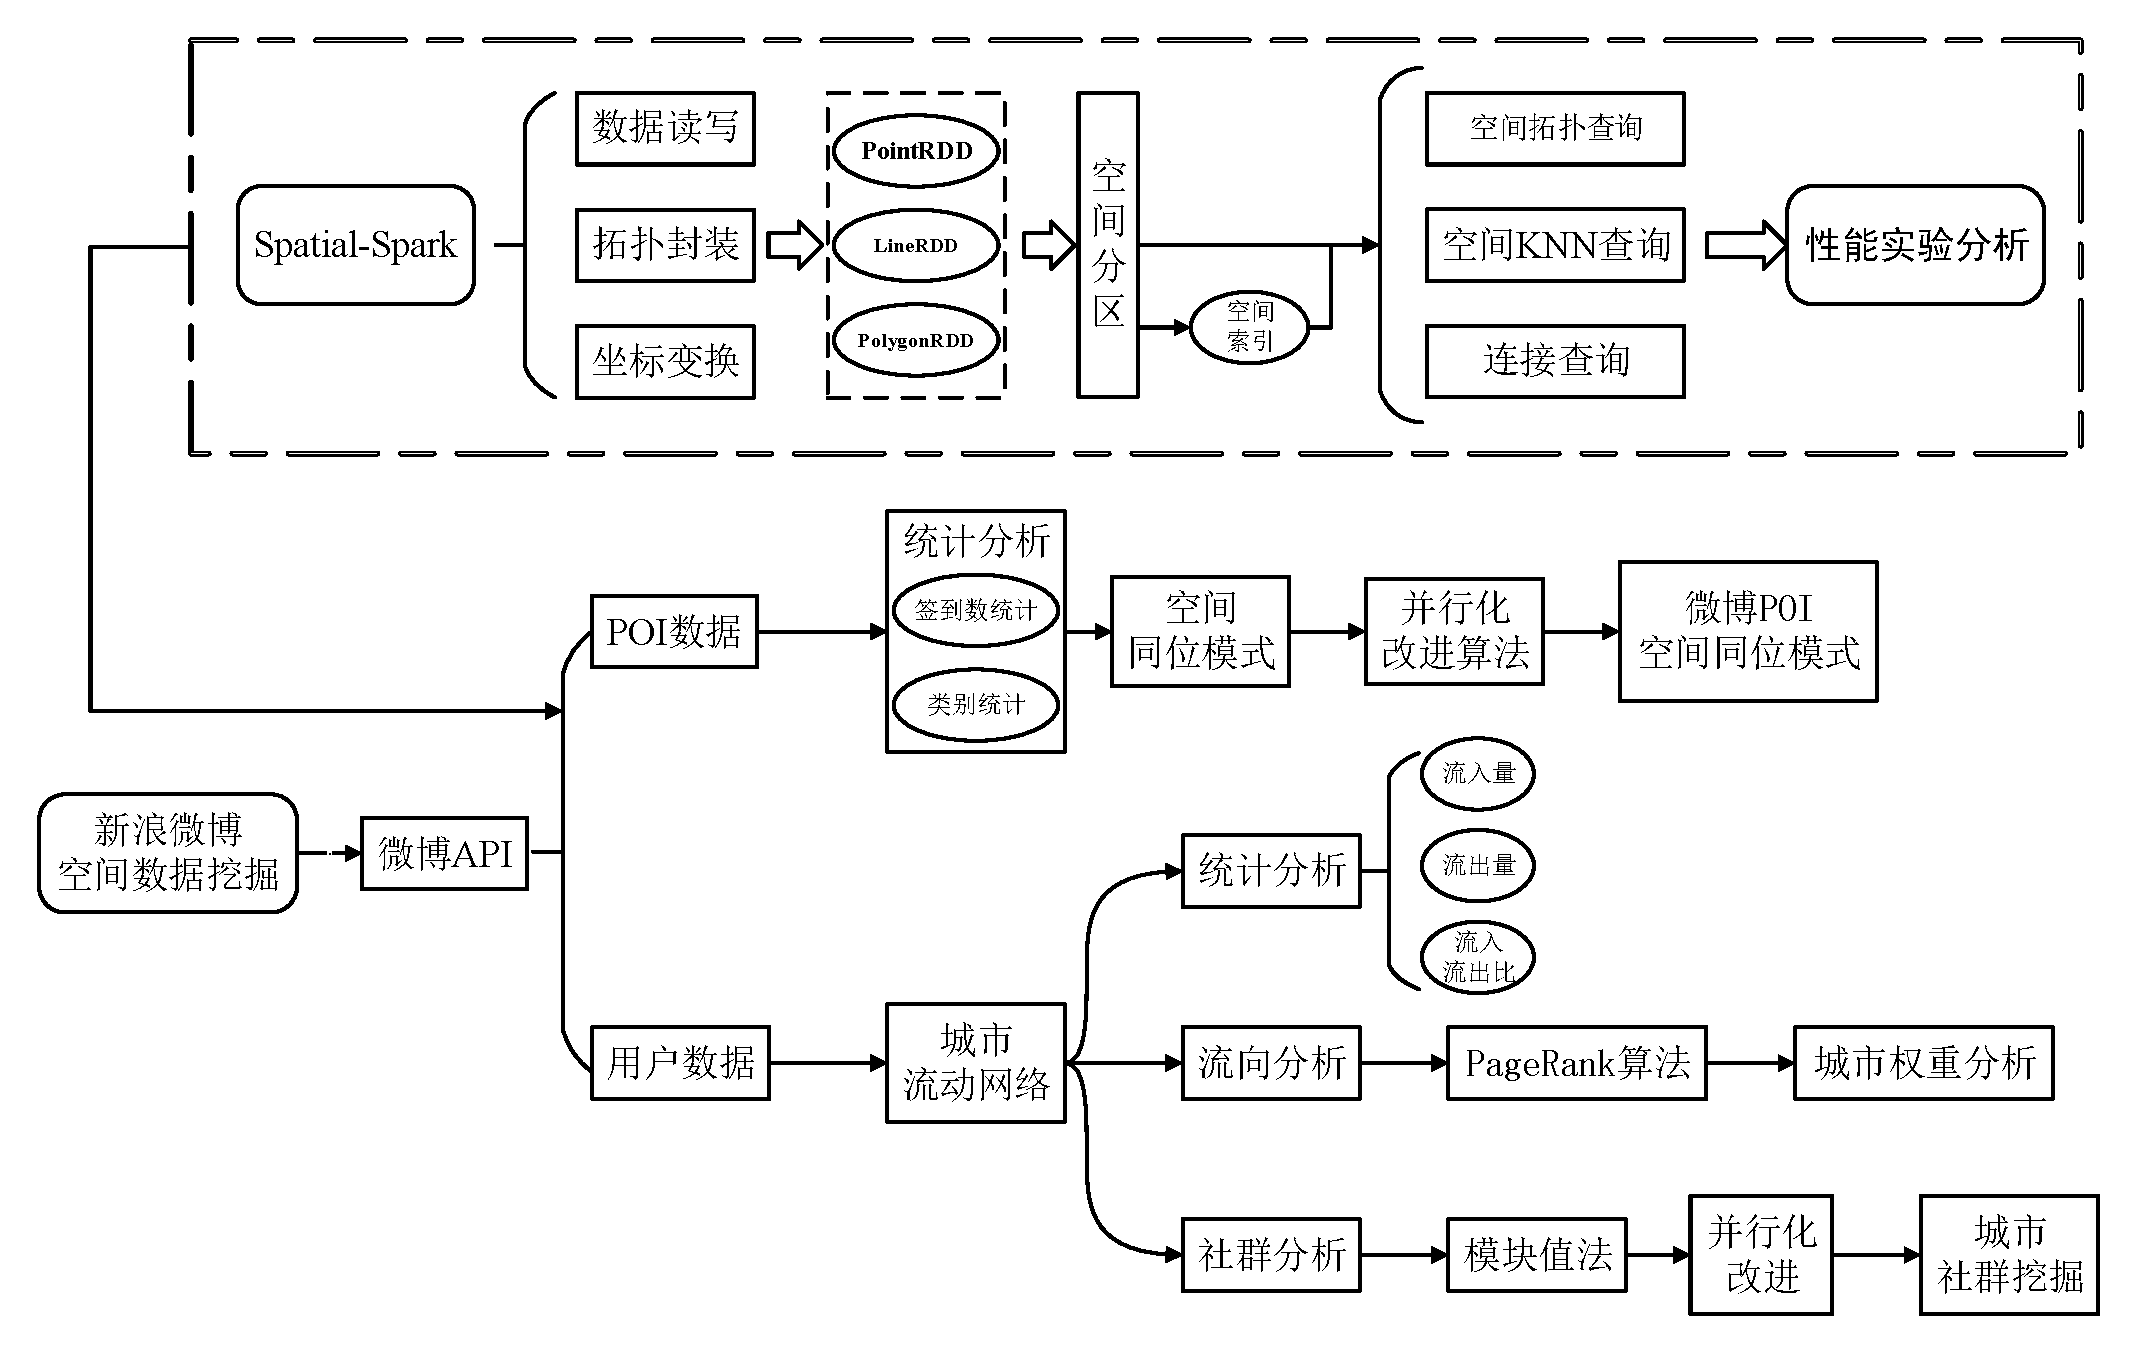
\includegraphics[scale=0.3]{figures/technology_route.pdf}
% \end{frame}
\section{绪论}

\begin{frame}{绪论}
    \begin{columns}
        \begin{column}{0.5\textwidth}
        \includegraphics[scale=0.3]{figures/smartcity.jpg}
        \end{column}

        \begin{column}{0.5\textwidth}
        \textbf{智慧城市:} 
        
        数字城市、物联网、云计算
        \vspace{2em}

        \pause
        \alert{数字城市}
        \begin{itemize}
        \item 空间信息快速获取技术
        \item 海量空间数据管理技术
        \item 空间信息可视化技术
        \item 空间数据分析挖掘技术
        \item 网络服务技术
        \end{itemize}
        \end{column}
   \end{columns}
\end{frame}

\begin{frame}{绪论}
    \textbf{移动互联网发展}

    \alert{LBS应用}
    打车软件、O2O软件、社交网络软件

    \vspace{2em}
    \pause
    \textbf{意义}
    \begin{itemize}
        \pause
        \item 对个人而言(智慧生活)
        \pause
        \item 对商业公司而言(智慧商业)
        \pause
        \item 对政府决策部门而言(智慧政府)
    \end{itemize}
\end{frame}

\begin{frame}[t]{绪论}
% \alert{海量数据处理}

% 业界使用Hadoop并行计算框架,但是存在处理速度慢、计算抽象层次较低等缺陷。

% \pause
% Spark是新型的并行计算框架,内存计算速度快,算子表现力丰富。但是对空间数据类型和空间数据操作支持不够。

\begin{columns}
    \begin{column}{0.4 \textwidth}

        \begin{center}
        \alert{海量数据处理}

        \vspace{1em}
        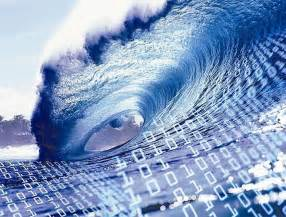
\includegraphics[height=3.5cm]{figures/seaamountdata.jpeg}
        \end{center}


    \end{column}

    \pause
    \begin{column}{0.6 \textwidth}

        \begin{center}
            \alert{并行计算}

            \vspace{1em}
            \includegraphics[height=3.5cm]{figures/parallelcomputation.png}
        \end{center}
       
    \end{column}

\end{columns}

% \vspace{2em}

% \pause
% \alert{并行化算法设计}

% 空间数据挖掘算法并没有针对并行化计算框架进行设计。

\end{frame}

\begin{frame}[c]{绪论}
    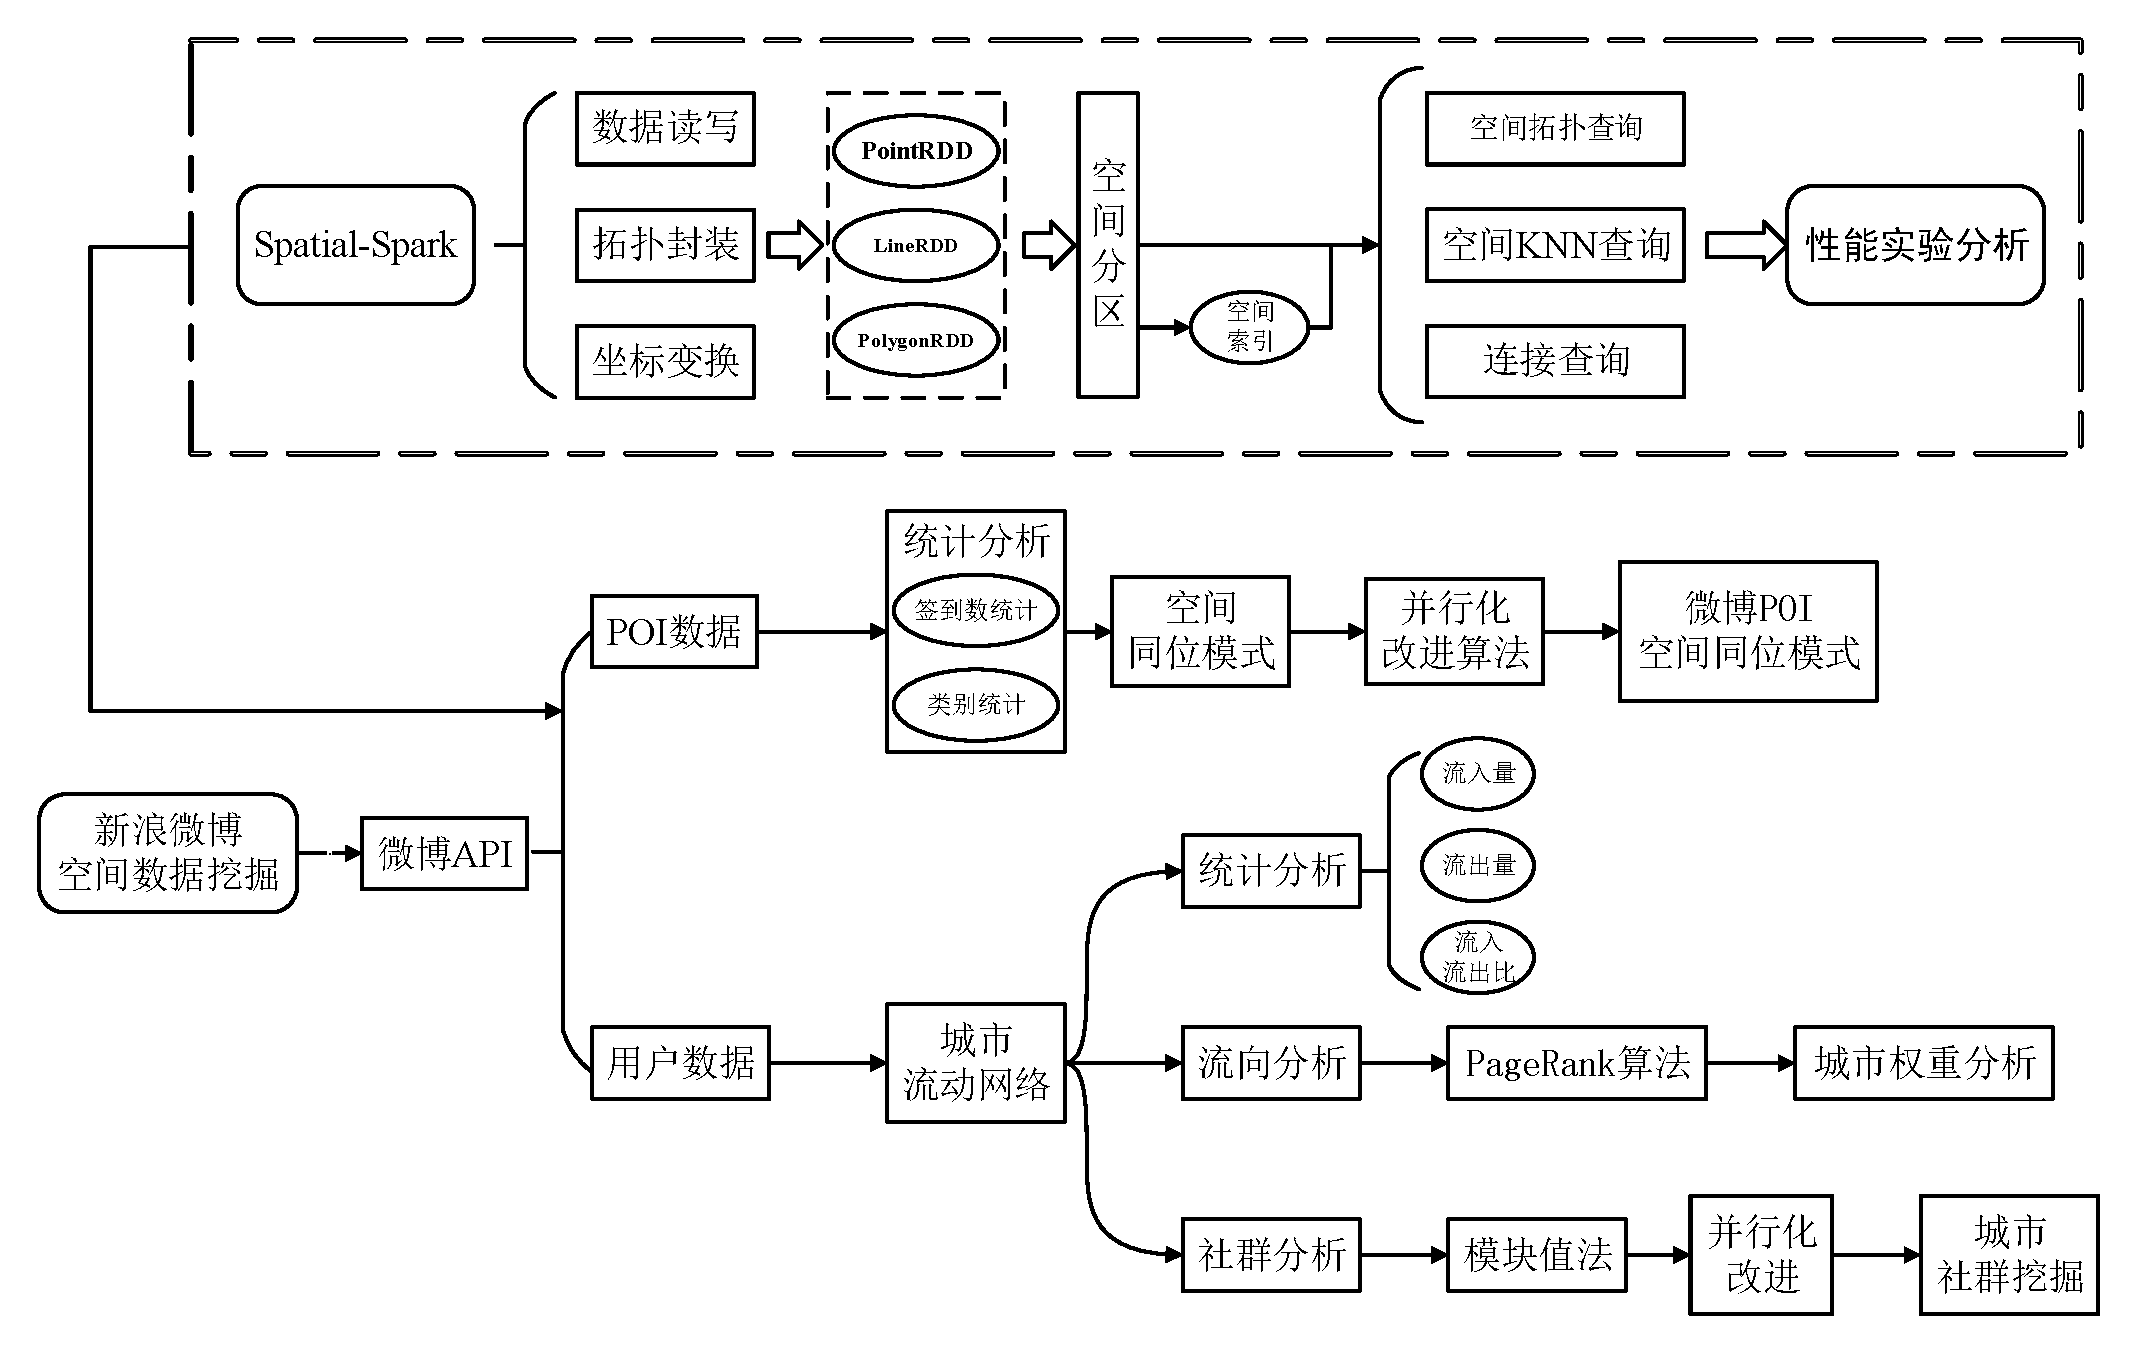
\includegraphics[scale=0.3]{figures/technology_route.pdf}
\end{frame}
\section{相关技术}

\subsection{Hadoop}

\begin{frame}[t]{相关技术(Hadoop)}
    \textbf{Hadoop}是Apache基金会推出的大数据计算平台
    
    \pause
    HDFS(Hadoop Distributed File System)

    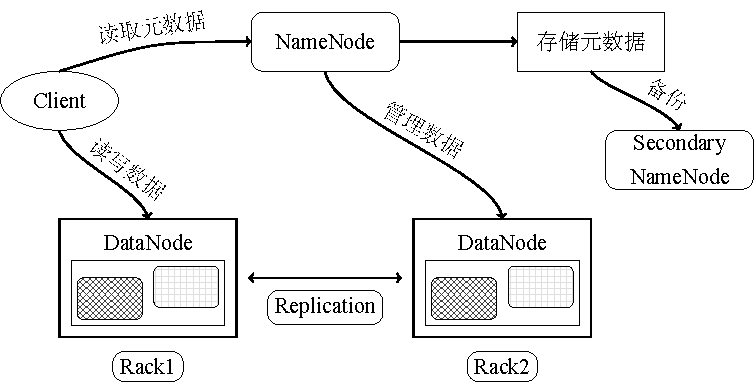
\includegraphics[scale=0.8]{figures/hdfs.pdf}
\end{frame}

\begin{frame}[t]{相关技术(Hadoop)}
    \textbf{Hadoop MapReduce}

    \pause
    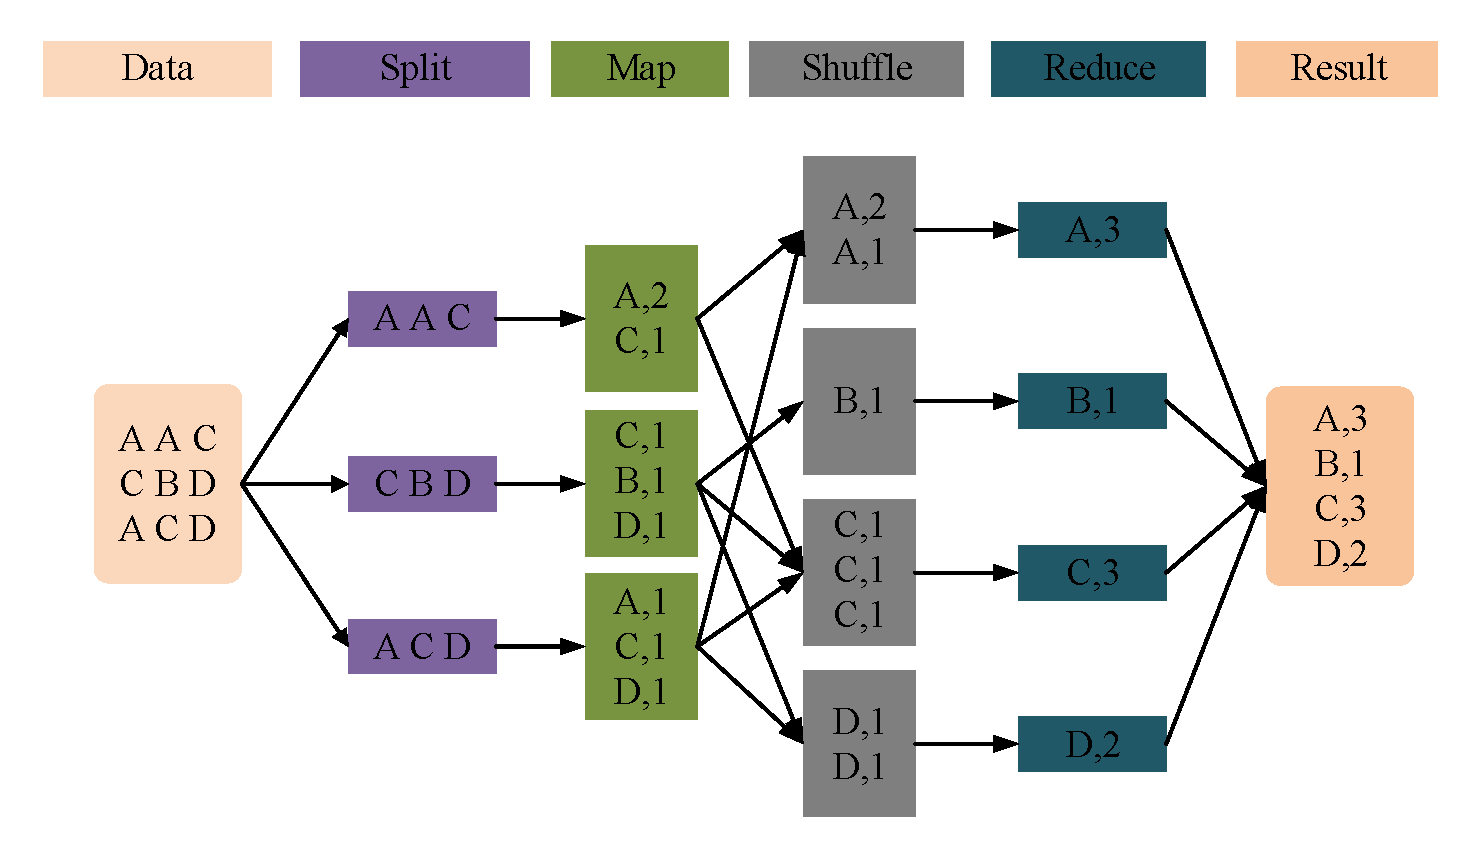
\includegraphics[scale=0.4]{figures/mapreduce.pdf}

    \pause
    \vspace{-1em}
    \begin{center}
    \alert{缺陷: }单点故障、算子抽象、IO操作频繁
    \end{center} 
\end{frame}

\subsection{Spark}

\begin{frame}[c]{相关技术(Spark)}
    \begin{columns}
        % one column
        \begin{column}{0.5 \textwidth}
            \textbf{Spark}技术生态系统。

            \vspace{0.5em}
            \begin{figure}
                \centering
                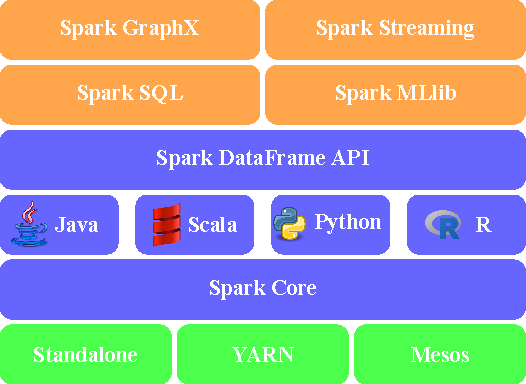
\includegraphics[scale=0.6]{figures/spark.pdf}
            \end{figure}            
        \end{column}

        %next column
        
        \pause
        \begin{column}{0.5 \textwidth}
            \begin{itemize}
                \item \textbf{Spark SQL}: 类SQL语言查询结构化数据
                \item \textbf{Spark MLlib}: 常用机器学习算法Spark实现
                \item \textbf{Spark GraphX}: 分布式图及其计算Spark实现
                \item \textbf{Spark Streaming}: Spark流应用计算框架
            \end{itemize}
        \end{column}
    \end{columns}
\end{frame}

\begin{frame}[t]{相关技术(Spark)}
    弹性分布式数据集(RDD)是Spark的核心抽象,在内存中已被分区、只读的、并提供
    一组丰富的操作方式的数据\textbf{集合}。

    \vspace{2em}
    \pause
    \alert{RDD算子}
    \begin{itemize}
        \item \textbf{Transformation} 
        \item \textbf{Action}
    \end{itemize}

\end{frame}

\begin{frame}[c]{相关技术(Spark)}
    \begin{columns}
        \begin{column}{0.5 \textwidth}
            Spark一栈式解决方案的\alert{优势:}
            
            \vspace{0.5em}
            \begin{itemize}
                \item 快速处理,内存计算
                \item 通用性,技术方案无缝集成
                \item 与Hadoop集群集成
            \end{itemize}
        \end{column}

        \pause
        \begin{column}{0.5 \textwidth}
            Spark在处理海量空间数据\alert{劣势:}

            \vspace{0.5em}
            \begin{itemize}
                \item 不支持空间数据类型
                \item 不支持空间操作
                \item 没有空间数据优化
            \end{itemize}
        \end{column}
    \end{columns}

\end{frame}

% \subsection{微博数据接口}

% \begin{frame}[c]{微博数据接口}
%     新浪微博提供了API方便第三方程序访问微博丰富的数据资源

%     \begin{figure}
%         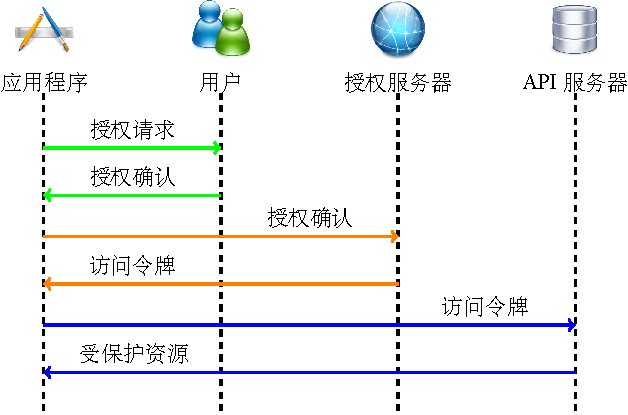
\includegraphics[scale=0.8]{figures/api.pdf}
%     \end{figure}
% \end{frame}

% \begin{frame}[t]{微博数据接口}
%     \alert{HTTP Get}请求

%     \vspace{0.5em}
%     \pause
%     \begin{itemize}
%     \item location/geo/address\_to\_geo $\rightarrow$  根据地址返回地理信息坐标 
%     \item location/pois/show\_batch $\rightarrow$ 批量获取POI点的信息
%     \item location/citycode $\rightarrow$ 城市代码对应表
%     \item place/nearby/pois $\rightarrow$ 获取附近的POI点
%     \end{itemize}
% \end{frame}


\section{Spatial-Spark}

\subsection{空间数据分析处理}

\begin{frame}[t]{Spatial-Spark}
    \begin{columns}
        %Transform and projection
        \begin{column}{0.4 \textwidth}

            \begin{center}
            \alert{Proj.4}

            \begin{itemize}
                \item 空间椭球基础
                \item 空间参照系统
                \item 空间投影系统
                \item 坐标换算
            \end{itemize}
            \end{center}
            
        \end{column}
        % JTS
        \pause
        \begin{column}{0.6 \textwidth}

            \begin{center}
             \alert{JTS Topogy Suite}

                \begin{itemize}
                \item 简单空间要素类型
                \item 空间数据分析和空间运算
                \item 空间数据读写
                \end{itemize}
            \end{center}
           
        \end{column}
    \end{columns}
\end{frame}

\subsection{RDD空间扩展}

\begin{frame}[c]{RDD空间扩展}
    \begin{center}
        \alert{Spatial-Spark体系结构}
    

    \vspace{1em}
    \begin{figure}
        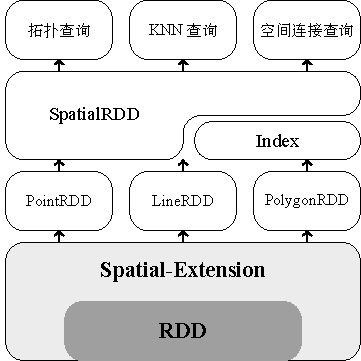
\includegraphics[scale=1.0]{figures/spatialspark.pdf}
    \end{figure}
    \end{center}
\end{frame}

\begin{frame}[c]{RDD空间扩展}
    PointRDD、LineRDD和PolygonRDD

    Spatial-RDD
    \pause
    \begin{itemize}
        \item HDFS中读取
    \end{itemize}
    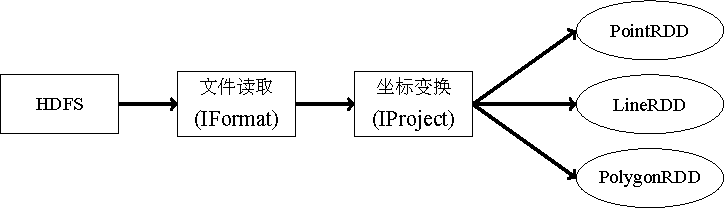
\includegraphics[scale=0.8]{figures/spatialRDD.pdf}

    \pause
    \begin{itemize}
        \item Spatial-RDD空间运算相互转换
    \end{itemize}
\end{frame}

\begin{frame}[c]{RDD空间扩展}
    \begin{columns}
        \begin{column}{0.6 \textwidth}
        R树空间索引

        \vspace{1em}
        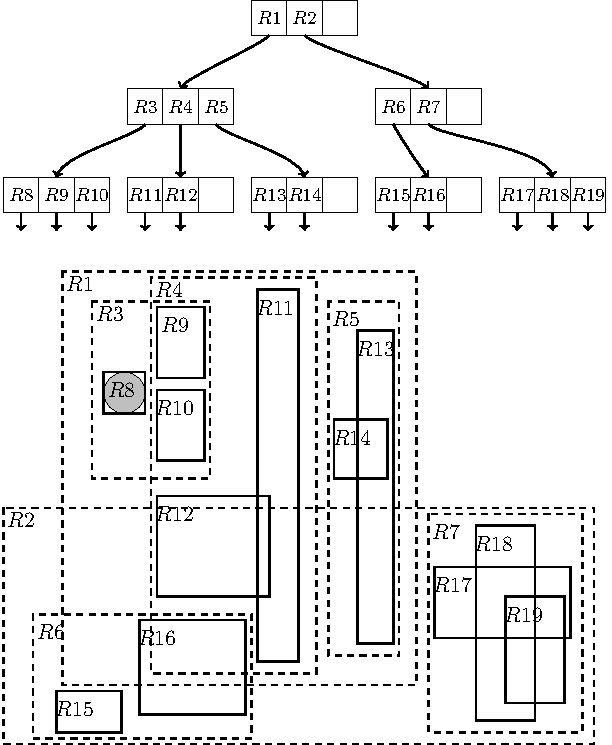
\includegraphics[scale=0.4]{figures/rtree.pdf}
        \end{column}

        \pause
        \begin{column}{0.4 \textwidth}
            \begin{itemize}
                \item R树插入
                \pause
                \item R树查询
                    \begin{itemize}
                        \pause
                        \item 过滤
                        \pause
                        \item 精选
                    \end{itemize}
            \end{itemize}
        \end{column}
    \end{columns}
\end{frame}

\begin{frame}[c]{RDD空间扩展}
    \begin{itemize}
        \item \alert{空间拓扑查询}
    \end{itemize}
    支持Spatial-RDD之间的所有拓扑操作

    \pause
    \begin{itemize}
        \item \alert{空间KNN查询}
    \end{itemize}
    借助优先级队列,筛选K个邻居;可借助索引加速空间查询

    \pause
    \begin{itemize}
        \item \alert{空间连接查询}
    \end{itemize}
    过滤步骤;精选步骤
\end{frame}
\subsection{实验分析}

\begin{frame}[t]{实验分析}
    MapReduce与Spatial-Spark空间过滤筛选对比
    \vspace{1em}
    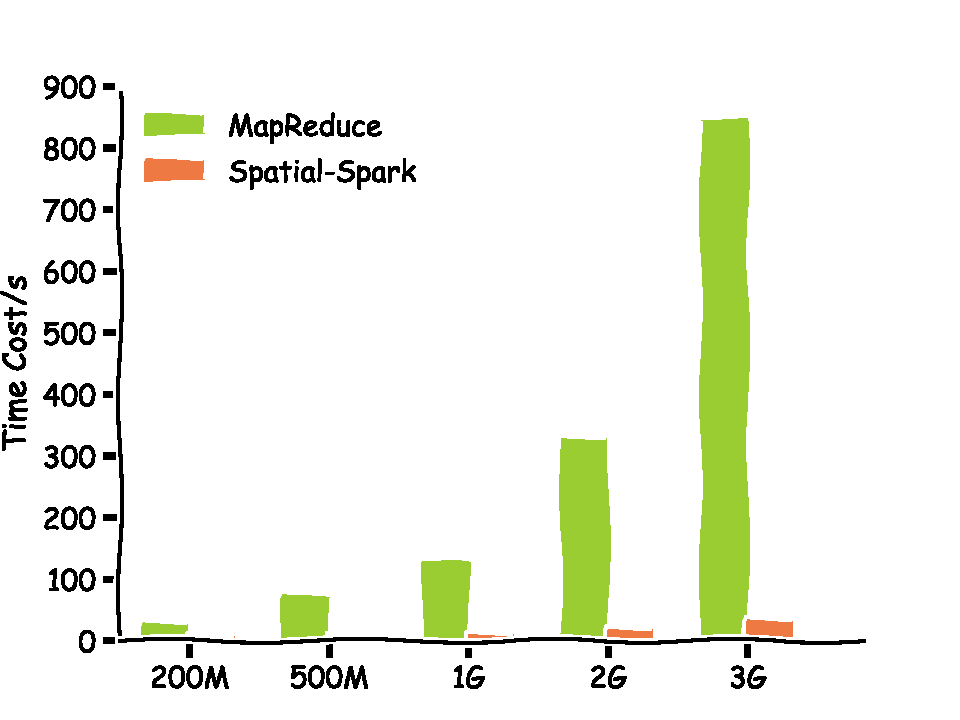
\includegraphics[width=0.9 \textwidth]{figures/topo_query.pdf}
\end{frame}

\begin{frame}[t]{实验分析}
    Spatial-Spark集群扩展性能分析
    \vspace{1em}
    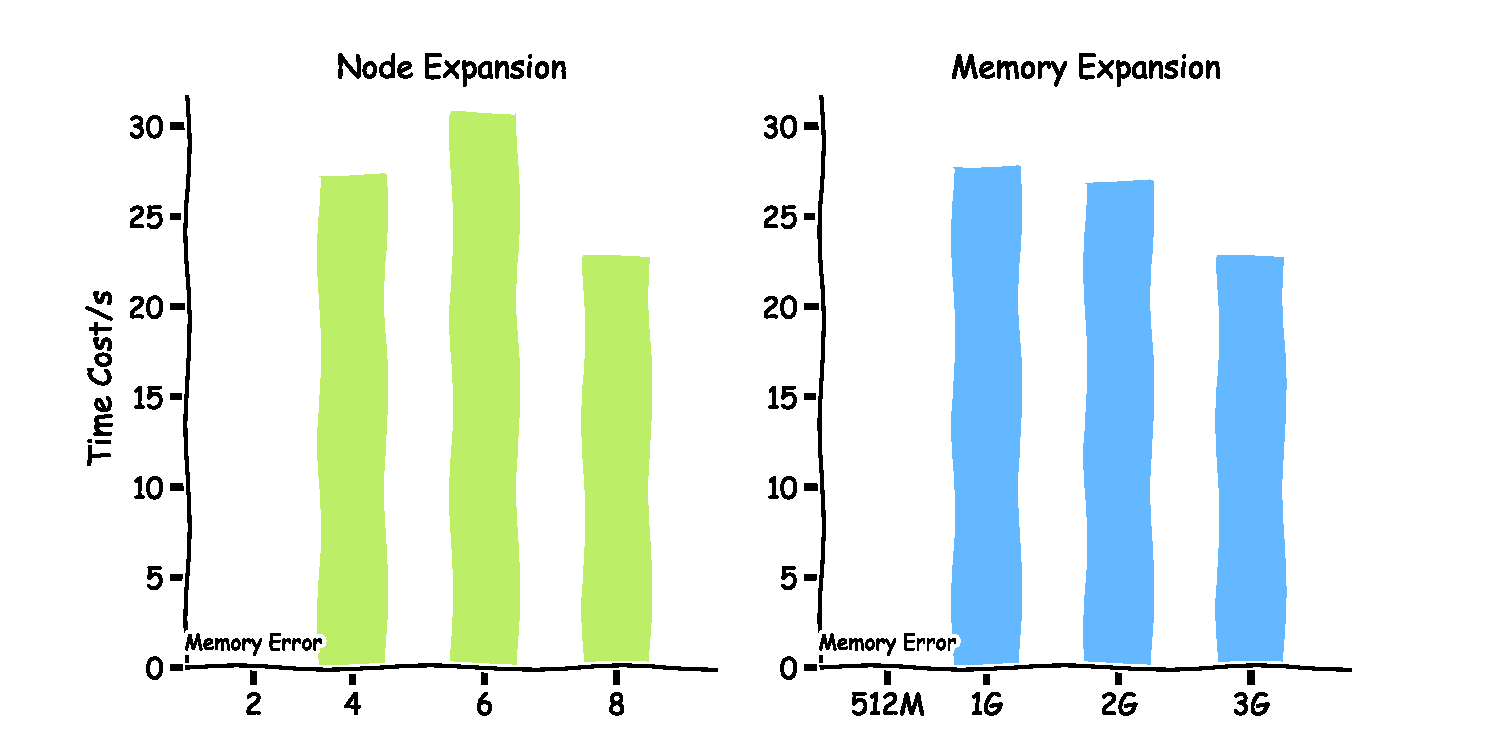
\includegraphics[width=0.9 \textwidth]{figures/node_memory.pdf}
\end{frame}

\begin{frame}[t]{实验分析}
    Spatial-Spark 空间索引性能分析
    \vspace{1em}
    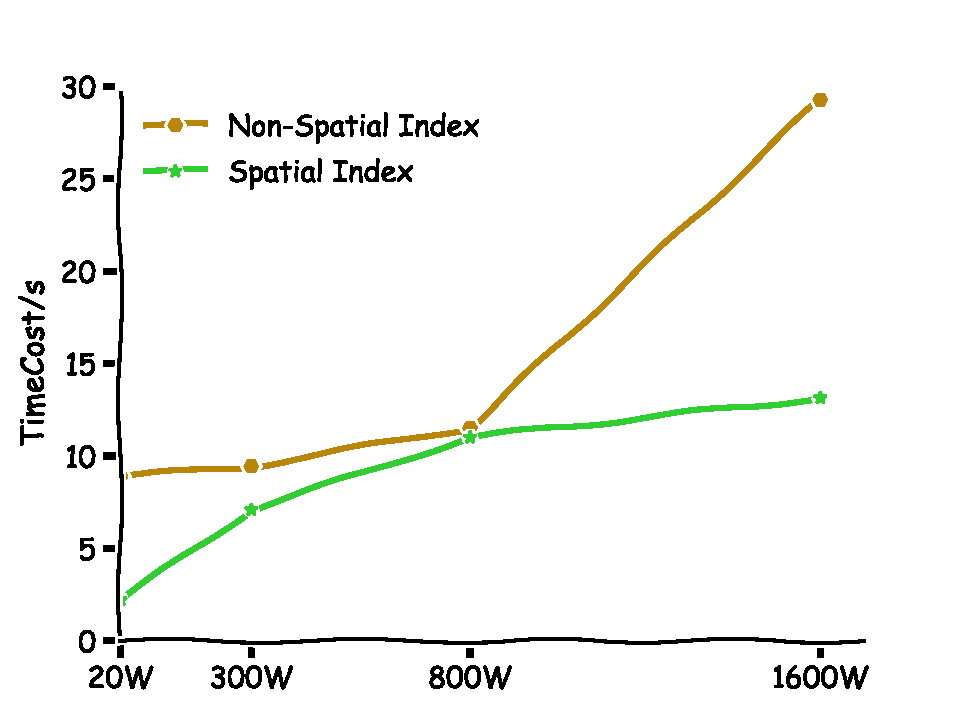
\includegraphics[width=0.9 \textwidth]{figures/index.pdf}
\end{frame}



\section{POI空间分析}

\subsection{POI获取}

\begin{frame}[c]{POI空间分析(获取)}
    POI是新浪微博用户在使用过程中自行添加附近的热门位置

    \vspace{1em}
    \includegraphics[scale=0.3]{figures/webpoi.png}
\end{frame}

\begin{frame}[c]{POI空间分析(获取)}
    \begin{columns}
        \begin{column}{0.5 \textwidth}
            \alert{place/nearby/pois}
            \vspace{1em}
            \begin{itemize}
                \item \textbf{Lat:} 纬度
                \item \textbf{Long:} 经度
                \item \textbf{Range:} 查询半径
            \end{itemize}
        \end{column}
        
        \pause
        \begin{column}{0.5 \textwidth}
            \begin{itemize}
                \item \alert{投影}

                Lambert 投影

                \pause
                \item \alert{栅格化}

                \vspace{0.5em}
                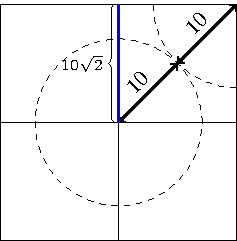
\includegraphics[scale=0.8]{figures/query.pdf}

                \pause
                \item \alert{坐标反算}

                适应API接口

            \end{itemize}
            
        \end{column}
    \end{columns}
\end{frame}

\subsection{统计分析}

\begin{frame}[c]{POI空间分析(统计)}
    \begin{columns}
        \vspace{0.5em}
        \begin{column}{0.5 \textwidth}
            \alert{热门签到地点}: sortBy, take

            \pause
            \begin{enumerate}
                \item 星光公益站
                \item 浦东机场
                \item 厦门高崎国际机场
                \item 中关村
                \item 深圳宝安机场
                \item 丽江古城
                \item 成都双流国际机场
                \item 望京
                \item 首都机场T3航站楼
                \item 广州白云机场
            \end{enumerate}
        \end{column}

        \pause
        \vspace{0.5em}
        \begin{column}{0.5 \textwidth}
            \alert{热门签到类别}: groupBy, reduce

            \pause
            \vspace{2em}
            \includegraphics[scale=0.4]{figures/poi_category.png}
        \end{column}
    \end{columns}
\end{frame}



\subsection{同位模式}

\begin{frame}[c]{POI空间分析(同位模式)}
    \alert{关联规则算法}

    \vspace{1em}
    \begin{itemize}
        \item 事务项$T$,由集合$I_1,I_2,\ldots,I_m$组成
        \item $P \in T, Q \in T$,规则$P \rightarrow Q$
        \item 置信度约束 $c(P \rightarrow Q) \ge min\_c$
        \item 支持度约束 $s(P \rightarrow Q) \ge min\_s$
    \end{itemize}

    \pause
    \vspace{1em}
    \alert{Apriori算法}

    \begin{itemize}
        \item 频繁项的子 集必须也是频繁的
        \item 非频繁项的超集必定非频繁
    \end{itemize}
\end{frame}

\begin{frame}[t]{POI空间分析(同位模式)}

    \begin{alert}{单主题空间关联规则}
     \begin{equation}
        P_1\wedge P_2\wedge \ldots \wedge P_m \rightarrow Q_1\wedge Q_2\wedge \ldots \wedge Q_n(s\%, c\%)
    \end{equation}
    \end{alert}
    % % 单主题空间关联规则
    
    \pause
    \begin{alert}{多主题同位模式}
            \begin{equation}
                R(a_1,b_1) \Leftrightarrow (distance(a_1,b_1)\le d)
            \end{equation}

            \pause
            \begin{figure}
                \centering
                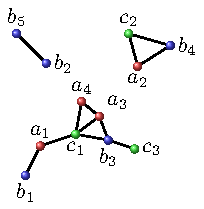
\includegraphics[scale=1.0]{figures/spatialrelation.pdf}
            \end{figure}
    \end{alert}

    % 其中$P_i$和$Q_j$中至少有一个为空间谓词
\end{frame}

% \begin{frame}[c]{POI空间分析(同位模式)}
%     多主题同位模式
%     \begin{equation}
%         R(a_1,b_1) \Leftrightarrow (distance(a_1,b_1)\le d)
%     \end{equation}

%     \pause
%     \begin{figure}
%         \centering
%         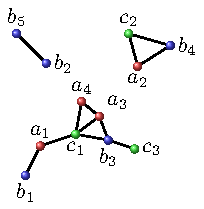
\includegraphics[scale=1.0]{figures/spatialrelation.pdf}
%     \end{figure}
% \end{frame}

\begin{frame}[c]{POI空间分析(同位模式)}
    \begin{columns}
        \begin{column}{0.3 \textwidth}
            \begin{figure}
                \centering
                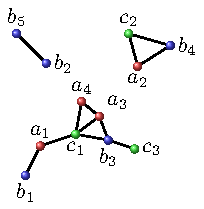
\includegraphics[scale=0.8]{figures/spatialrelation.pdf}
            \end{figure}
        \end{column}

        \begin{column}{0.7 \textwidth}
            \alert{参与率}
            \begin{equation}
                PR(c,f_i)=\frac{|\pi_{f_i}(table\_instance(c))|}{|table\_instance(\{f_i\})|}
            \end{equation}
            $PR(\{A,B,C\},A)=2/4=0.5$
            
            $PR(\{A,B,C\},B)=2/5=0.4$
            
            $PR(\{A,B,C\},C)=2/3=0.67$

            \pause
            \vspace{0.5em}
            \alert{参与度}
            \begin{equation}
                PI(c)=min_{i=1}^{k}\{PR(c,f_i)\}
            \end{equation}

            $PI(\{A,B,C\})=min(0.5,0.4,0.67)=0.4$
        \end{column}
    \end{columns}
\end{frame}

\begin{frame}[t]{POI空间分析(同位模式)}
    Spatial-Saprk二阶模式生成

    \vspace{1em}
    \begin{figure}
        \centering
        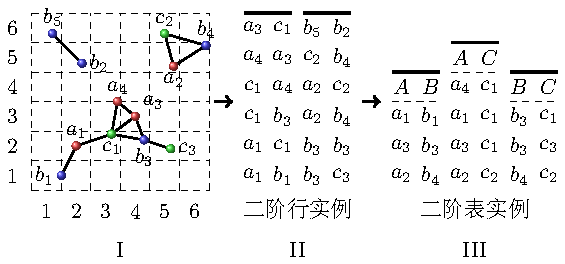
\includegraphics[scale=0.6]{figures/two_order.pdf}
    \end{figure}
    

    \pause
    键值相等判断
    \begin{figure}
        \centering
        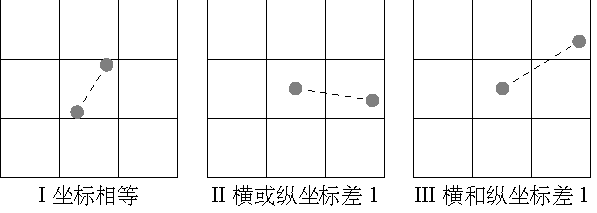
\includegraphics[scale=0.5]{figures/keyequal.pdf}
    \end{figure}
  
\end{frame}

\begin{frame}[t]{POI空间分析(同位模式)}

% \begin{algorithm}[H]
% \begin{algorithmic}[1]
% \FOR{$i=1$ to $N$}
% \FOR{$j=1$ to $JJJJ$}
% \STATE $energy[i*JJJ+j] =$ 
% $ interpolate(AAA[i*JJJ+j], ZZZ)$
% \ENDFOR
% \ENDFOR
% \end{algorithmic}
% \caption{pseudocode for the calculation of }
% \label{alg:seq}
% \end{algorithm}
\begin{algorithm}[H]
\tiny
\caption{co-location算法}
\begin{algorithmic}[1]   
\REQUIRE  ~~\\  
点集:points;\\  
距离阈值:d;\\
参与率阈值:threshold;\\  
\ENSURE ~~\\  
空间同位模式:colocation patterns; \\
\pause
\STATE $P_2$ = Spatial-Spark.join(points, d, threshold)
\WHILE{$P_k$ is not empty and $k$ < N} 
\pause
\STATE // \alert{Join操作,RowPattern重写}
\STATE $C_{k+1}$ = gen\_candinate\_cocolation($P_k$,$k$) $//$k+1阶候选集合
\pause
\STATE // \alert{距离阈值比较}
\STATE $C_{k+1}$ = pruning($C_{k+1}$, $d$)
\pause
\STATE // \alert{reduce生成表实例}
\STATE $T_{k+1}$ = gen\_table\_ins()$//$生成表实例
\pause
\STATE // \alert{threshold 筛选}
\STATE $P_{k+1}$ = Select\_Colocation\_Pattern($T_{k+1}$, threshold) $//$ 筛选表实例
\pause
\STATE $k$ = $k+1$ $//$下一轮迭代
\pause
\ENDWHILE 
\pause
\RETURN $P_2$,$\dots$,$P_k$
\end{algorithmic}
\end{algorithm} 
\end{frame}


\begin{frame}[c]{POI空间分析(同位模式)}
    \scriptsize
    \begin{columns}
        \begin{column}{0.333 \textwidth}
        \alert{上海市}

        \vspace{1em}
        (高等院校,校园生活):0.556

        \vspace{1em}
        (高等院校,日本料理):0.472

        \vspace{1em}
        (高等院校,西餐厅):0.454
        \vspace{1em}

        (高等院校,甜品店):0.451
        \vspace{1em}

        (高等院校,培训机构):0.446
        \vspace{1em}

        (高等院校,医院):0.443
        \vspace{1em}

        (高等院校,糕饼店):0.441
        \vspace{1em}

        (高等院校,餐饮美食):0.432
        \end{column}

        \begin{column}{0.333 \textwidth}
        \alert{武汉市}
        \vspace{1em}

        (高等院校,校园生活):0.531
        \vspace{1em}

        (高等院校,图书馆):0.528
        \vspace{1em}

        (高等院校,糕饼店):0.384
        \vspace{1em}

        (高等院校,快餐厅):0.368
        \vspace{1em}

        (高等院校,四川菜):0.361
        \vspace{1em}

        (高等院校,火锅店):0.358 
        \vspace{1em}

        (高等院校,连锁酒店):0.354
        \vspace{1em}

        (高等院校,医院):0.328
        \end{column}

        \begin{column}{0.333 \textwidth}
        \alert{重庆市}

        \vspace{1em}
        (高等院校,校园生活):0.306
        \vspace{1em}

        (高等院校,ATM):0.238
        \vspace{1em}

        (高等院校,科研机构):0.224
        \vspace{1em}

        (高等院校,图书馆):0.224
        \vspace{1em}

        (高等院校,超市):0.217
        \vspace{1em}

        (高等院校,特色餐厅):0.215
        \vspace{1em}

        (高等院校,电子卖场):0.210
        \vspace{1em}

        (高等院校,KTV):0.205
        \end{column}
        
    \end{columns}
\end{frame}

\begin{frame}[c]{POI空间分析(同位模式)}
    \alert{(高等院校, 培训机构)}

    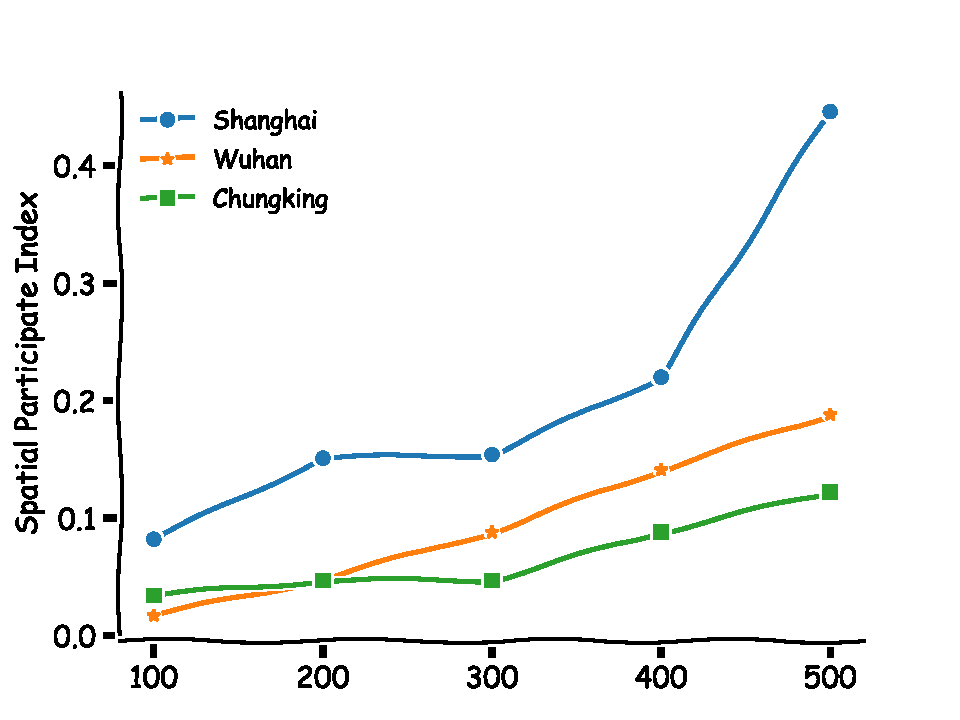
\includegraphics[scale=0.6]{figures/Participate.pdf}
\end{frame}

\begin{frame}[c]{POI空间分析(同位模式)}
    北京市POI空间模式,$d=500$m,空间参与度阈值为$0.6$

    \begin{itemize}
        \footnotesize
        \pause
        \item \textbf{二阶(29)}

        (中餐厅,校园生活),(校园生活,医院),(甜品店,中餐厅),(咖啡厅,校园生活),(咖啡厅,酒吧),(清真餐馆,酒吧) $\ldots$

        \pause
        \item \textbf{三阶(29)}

        (中餐厅,校园生活,医院),(电影院,KTV,美容美发店),
        (甜品店,中餐厅,美容美发店),(美容美发店,酒吧,甜品店),(中餐厅,校园生活,咖啡厅) $\ldots$

        \pause
        \item \textbf{四阶(19)}

        (电影院,KTV,咖啡厅,美容美发店),(KTV,中餐厅,甜品店,美容美发店),
        (甜品店,中餐厅,咖啡厅,美容美发店),(甜品店,咖啡厅,美容美发店,酒吧)$\ldots$

        \pause
        \item \textbf{五阶(7)}

        电影院,KTV,咖啡厅,甜品店,美容美发店),(KTV,中餐厅,咖啡厅,美容美发店,酒吧),
        (甜品店,中餐厅,咖啡厅,美容美发店,酒吧)$\ldots$

        \pause
        \item \textbf{六阶(1)}

        (KTV,中餐厅,咖啡厅,甜品店,美容美发店,酒吧)
    \end{itemize}
\end{frame}
\section{人口流动网络分析}

\subsection{数据获取}

\begin{frame}[c]{人口流动网络分析(获取)}
    \alert{人口流动}

    \textbf{place/nearby/users}

    \vspace{1em}
    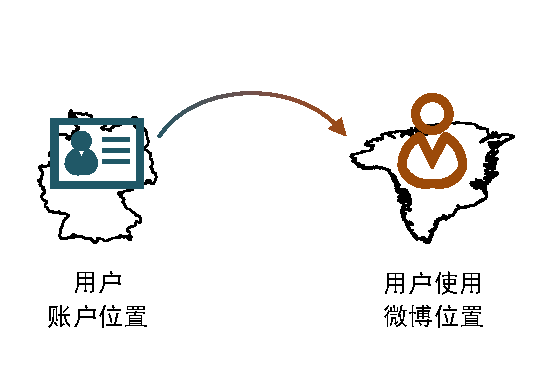
\includegraphics[scale=0.8]{figures/floating.pdf}

\end{frame}

\begin{frame}[t]{人口流动网络分析(获取)}
    \textbf{城市之间GraphX构建}

    \vspace{1em}
    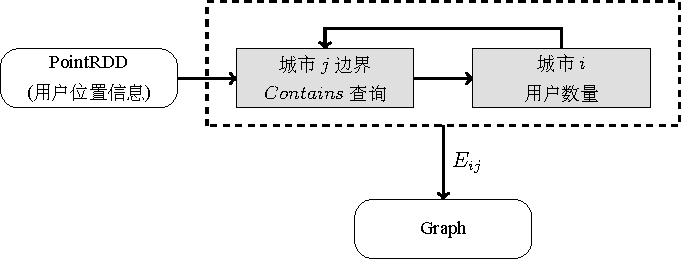
\includegraphics[scale=0.8]{figures/graph.pdf}
\end{frame}

\subsection{统计分析}

\begin{frame}[c]{人口流动网络分析(统计)}
    \begin{columns}
        \begin{column}{0.4 \textwidth}
            人口流动指数

            \begin{itemize}
                \item \textbf{流入量:} $\delta_i$
                \item \textbf{流出量:} $\omega_i$
                \item \textbf{流入流出比:} $\psi_i=\delta_i / \omega_i$
            \end{itemize}
        \end{column}

        % algorithm
        \pause
        \begin{column}{0.6 \textwidth}
            Graph并行化设计, aggreateMessages

            \vspace{0.5em}
            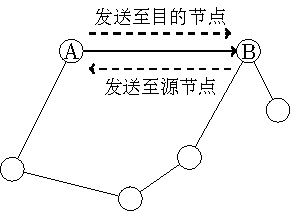
\includegraphics[scale=0.8]{figures/triplet.pdf}
        \end{column}
    \end{columns}
\end{frame}

\begin{frame}[t]{人口流动网络分析(统计)}
    全国城市人口流动情况

    \vspace{0.5em}
    \includegraphics[width=1.0 \linewidth]{figures/flowratio.png}

    \vspace{0.5em}
    \pause
    人口流动量前20\%的城市占全国总流动人口的70.1\%。
\end{frame}
%--- Next Frame ---%

\begin{frame}[t]{人口流动网络分析(统计)}
    人口流入流出比
    
    \begin{itemize}
        \pause
        \item \alert{大于1}

        辽源、鄂州、西双版纳、毕节、永州、七台河、娄 底、姿阳、白色、黄冈、松原、三亚、娄底、大理等

        \pause
        \item \alert{接近1}

        上海、北京、成都、武汉、哈尔滨、嘉兴、杭州、长 沙,广州、西安、太原、郑州、沈阳、乌鲁木齐等

        \pause
        \item \alert{小于1}

        东莞、马鞍山、芜湖、青岛、苏州、深圳、包头、宁 波、无锡、唐山,石家庄、呼和浩特等
    \end{itemize}
\end{frame}
%--- Next Frame ---%

\subsection{流向分析}

\begin{frame}[t]{人口流动网络分析(流向分析)}
    \begin{columns}
        \begin{column}{0.4 \textwidth}
            \alert{流向示意图}

            \begin{figure}
                \includegraphics[scale=0.4]{figures/flow.jpg}
            \end{figure}
        \end{column}

        \pause
        \begin{column}{0.6 \textwidth}
            \textbf{PageRank}计算网络节点的权重

            \begin{enumerate}
                \item 北京 0.058
                \item 成都 0.033
                \item 上海 0.031
                \item 西安 0.028
                \item 广州 0.026
                \item 武汉 0.024
                \item 杭州 0.017
                \item 郑州 0.016
                \item 深圳 0.015
                
                $\ldots$
            \end{enumerate}
        \end{column}
    \end{columns}
\end{frame}


\begin{frame}[t]{人口流动网络分析(流向分析)}
    城市权重与城市GDP相关系数为0.8

    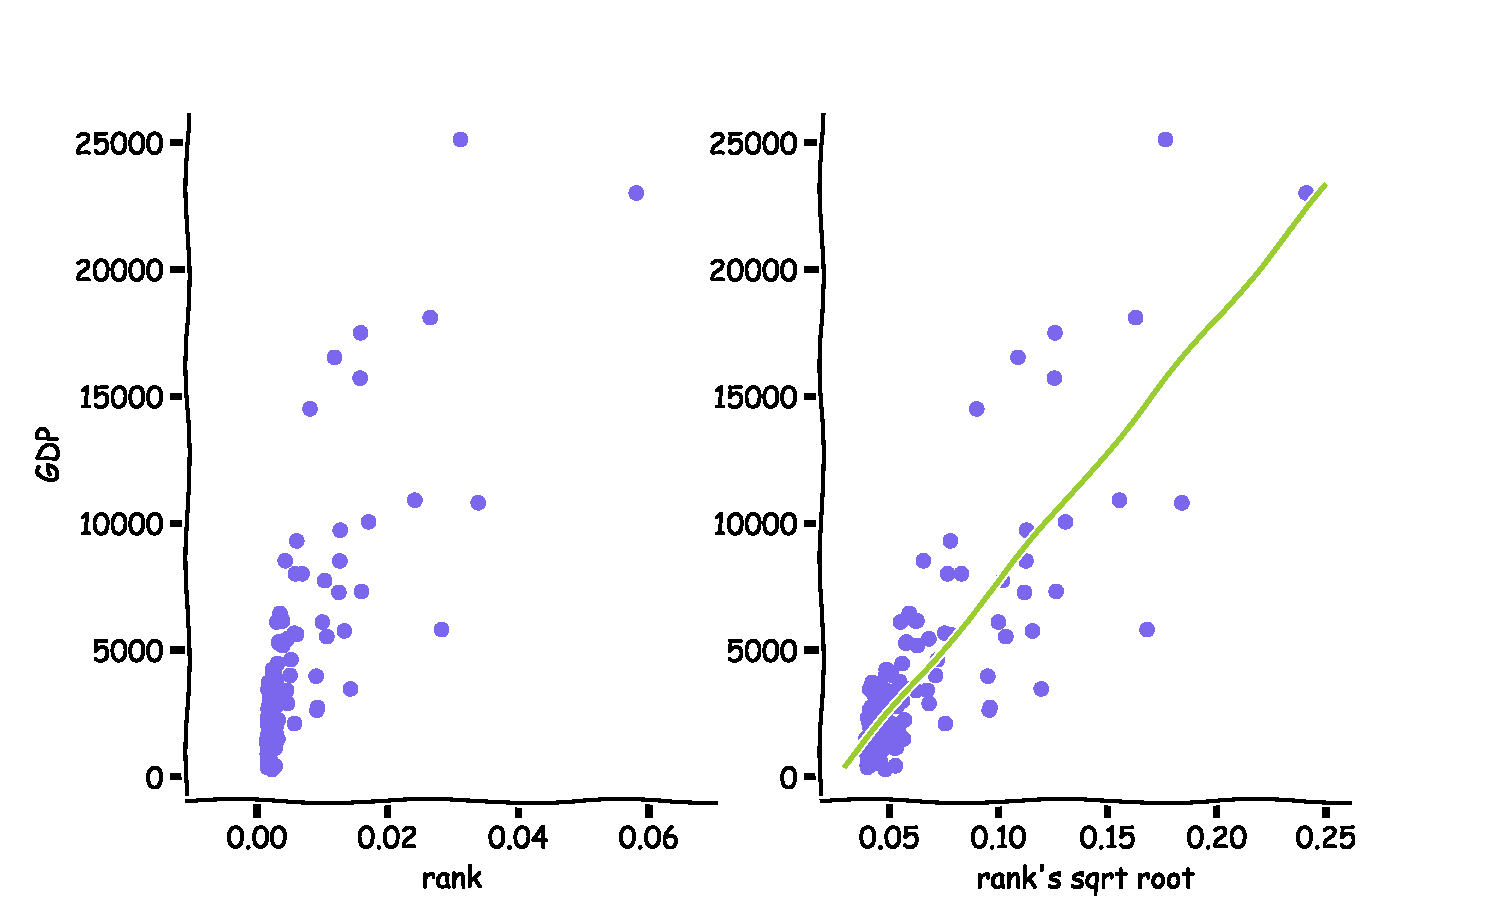
\includegraphics[scale=0.4]{figures/rank_gdp_scatter.pdf}

    $\text{GDP} = 1.037\times 10^5 rank^{0.5}-2669$
\end{frame}

\begin{frame}[t]{人口流动网络分析(流向分析)}
    残差平方与杠杆值散点图

    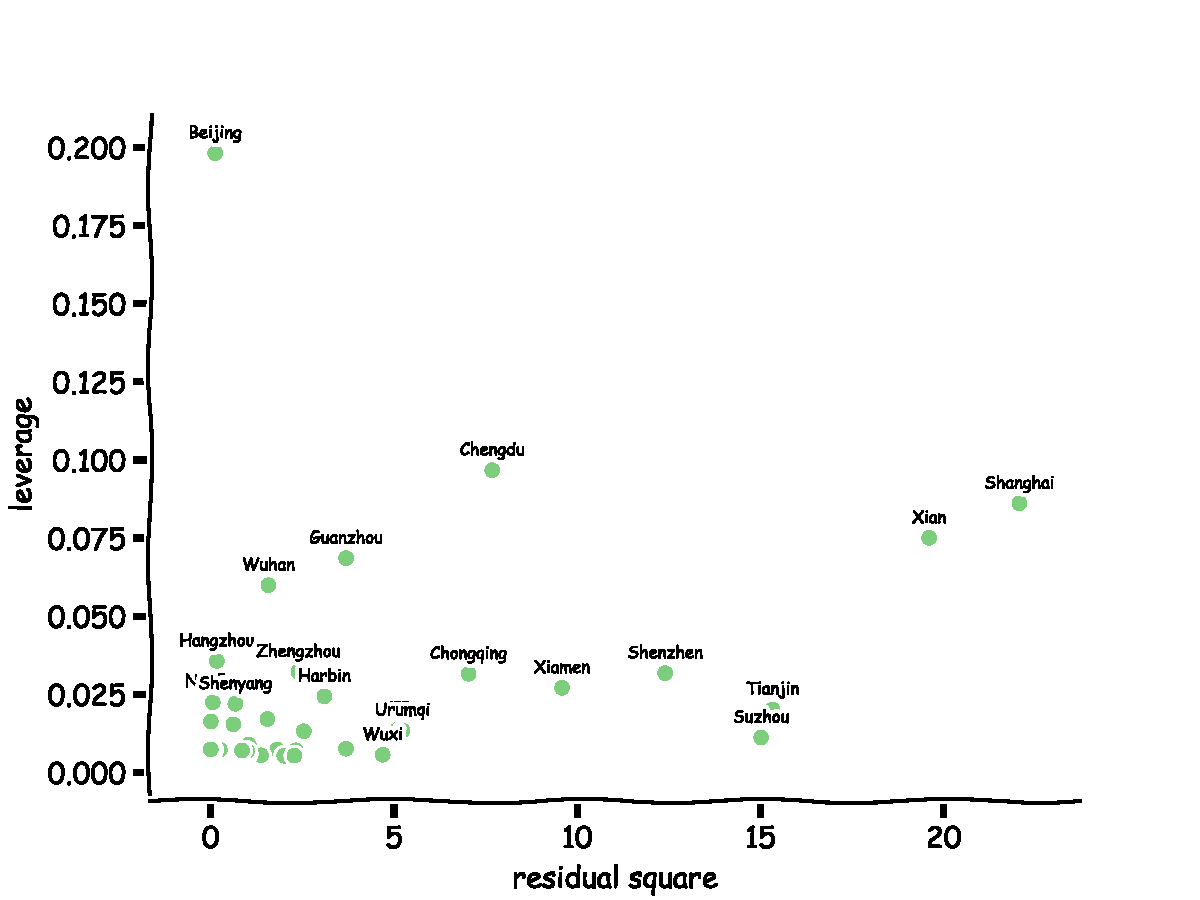
\includegraphics[scale=0.4]{figures/leverage.pdf}
\end{frame}

\begin{frame}[t]{口流动网络分析(流向分析)}
    \alert{结论}

    \begin{enumerate}
        \pause
        \item \textbf{城市权重与城市经济发展相对一致性}

        城市的权重与城市GDP呈现一定的正相关关系,即城市的权重越高,城市的GDP数值会高,但也有异常

        \pause
        \item \textbf{城市权重在流动网络层级分布}

        北京为第一个层级;成都、上海、西安、广州和武汉为第二层级;杭州、郑州、深圳、重庆
        和厦门为第三个层级;哈尔滨、南京、长沙、沈阳和天津为第三层级;

        \pause
        \item \textbf{东部城市与中西部城市权重的差异明显}

        东部城市群在人口流动网络中扮演重要的角色
    \end{enumerate}
\end{frame}
%--- Next Frame ---%



\subsection{社群挖掘}

\begin{frame}[t]{人口流动网络分析(社群挖掘)}
    \small

    \begin{alert}{模块值}
        \begin{equation}
            Q=\frac{1}{2m}\displaystyle{\sum_{vw}\big(W_{vw}-P_{vw}\delta(C_v,C_w)\big)}
        \end{equation}
    \end{alert}
    其中$W_{vw}$为网络中节点$v$和节点$w$之间的权重;$m$为权重之和;$P_{vw}$为零模型中节点之间的期望权重;$C_v$表示节点$v$所属的社群
的类别,如果节点$v$和节点$w$所属同一个社群,则$\delta(C_v,C_w)$为1,否则为0

    \begin{alert}{模块值更新}
        \begin{equation}
        \Delta Q_{AB}=Q_{AB}-Q_{A}-Q_{B}=\frac{1}{2m}\displaystyle{\sum_{a_i \in A, b_j \in B}}\bigg\{ \big( A_{ij} - \frac{k_ik_j}{2m} 
        \big) \times \delta \big[ r(i),r(j) \big] \bigg\}
        \end{equation}
    \end{alert}
%     将复杂网络划分若干个子社群

%     \pause
%     \alert{模块值法}

%     \begin{equation}
%         Q=\frac{1}{2m}\displaystyle{\sum_{vw}\big(W_{vw}-P_{vw}\delta(C_v,C_w)\big)}
%     \end{equation}

%     其中$W_{vw}$为网络中节点$v$和节点$w$之间的权重;$m$为权重之和;$P_{vw}$为零模型中节点之间的期望权重;$C_v$表示节点$v$所属的社群
% 的类别,如果节点$v$和节点$w$所属同一个社群,则$\delta(C_v,C_w)$为1,否则为0。

%     \pause
%     \alert{模块值更新}

%     \begin{equation}
%         \Delta Q_{AB}=Q_{AB}-Q_{A}-Q_{B}=\frac{1}{2m}\displaystyle{\sum_{a_i \in A, b_j \in B}}\bigg\{ \big( A_{ij} - \frac{k_ik_j}{2m} 
%         \big) \times \delta \big[ r(i),r(j) \big] \bigg\}
%     \end{equation}
\end{frame}
%--- Next Frame ---%

\begin{frame}[t]{人口流动网络分析(社群挖掘)}
    \emph{改进}

    \begin{equation}
        Q=\sum_{c}\big\{\frac{\sum_{in}}{2m} - (\frac{\sum_{tot}}{2m})^2\big\}
    \end{equation}

    其中$\sum_{in}$是社群$c$内部相互连接权重和,$\sum_{tot}$该社群$c$外部连接权重和

    \pause

    \begin{equation}
        \Delta Q=\big[ \frac{\sum_{in} + k_{i,in}}{2m} -(\frac{\sum_{tot}+k_i}{2m})^2 \big] 
            - \big[ \frac{\sum_{in}}{2m} - (\frac{\sum_{tot}}{2m})^2 - (\frac{k_i}{2m})^2 \big]
    \end{equation}

\end{frame}
%--- Next Frame ---%

\begin{frame}[t]{人口流动网络分析(社群挖掘)}

    \begin{algorithm}[H]
    \tiny
\caption{社群挖掘算法}
\begin{algorithmic}[1]
\REQUIRE ~~\\
网络图:graph; \\
最多迭代次数: maxIterations;\\
模块值变化阈值: modularityThreshold;\\
\ENSURE ~~\\
模块值最大社群图: graph; \\
\STATE 初始化$C_i,\{i=1, 2,\ldots , N\}$
\STATE iterate=0
\WHILE{changeRate<modularityThreshold || iteration < maxIterations}
    \STATE changeRate=0
    \FORALL{$i$ in graph.vertexs} 
    \STATE $Q_i=[\quad ]$
    \FORALL{$j$ in $i$ neighbors}
    	\STATE $Q_i$ += $\Delta Q(i,j)$ $//$计算模块值增益
    \ENDFOR
    \STATE $Q_{max}$=max($Q_i$)
    \IF {$Q_{max} > 0$}
    	\STATE graph=updategraph() $//$如果最大模块值增益大于零,合并顶点
	\STATE changeRate= $Q_{max}$
    \ENDIF
    \ENDFOR
 \STATE iterate += 1 \\
\ENDWHILE
\RETURN graph
\end{algorithmic}
\end{algorithm}
\end{frame}
%--- Next Frame ---%

\begin{frame}[t]{人口流动网络分析(社群挖掘)}
    并行化设计,aggregateMessages接口
    \begin{enumerate}

    \pause 
    \item \textbf{map阶段}

    消息类,包含了顶点、所属社群和目标社群的权重

    \pause
    \item \textbf{Reduce阶段}

    将发送到同一个顶点的消息按照模块增益值最大进行合并

    \pause
    \item \textbf{连通量合并}

    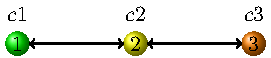
\includegraphics[scale=0.8]{figures/communitycombine.pdf}

    \pause
    \item \textbf{图更新}
    
    与上一轮的Graph对象的顶点进行joinVertice操作

    \end{enumerate}

\end{frame}
%--- Next Frame ---%

\begin{frame}[t]{人口流动网络分析(社群挖掘)}
    全国城市社群划分

    \includegraphics[scale=0.7]{figures/commumity.jpg}
\end{frame}
%--- Next Frame ---%

\begin{frame}[t]{人口流动网络分析(社群挖掘)}
    \alert{社群划分结果}

    \begin{enumerate}
        \item 北京、天津、河北城市、东三省城市、福建城市、三亚等
        \item 山东城市
        \item 河南城市
        \item 山西城市
        \item 湖北城市、江西城市
        \item 上海、江苏城市、安徽城市、浙江城市、丽江
        \item 广东城市、广西城市、湖南城市等
        \item 重庆、四川城市、贵州城市等西南城市
        \item 新疆城市、甘肃城市等西北城市
    \end{enumerate}
\end{frame}
%--- Next Frame ---%

\begin{frame}[t]{人口流动网络分析(社群挖掘)}
    \textbf{结论}

    \begin{enumerate}
        \item 城市之间人口流动以省份为划分的特征较为明显
        \item 城市社群组成受地理空间位置影响较大,有明显的区域特征
        \item 城市社群组成也存在不受地理位置影响的特殊情况,如福建省的城市与北方城市组成同一社群,从侧面表
              明其人口流动突破了地理空间的限制
        \item 当对全国社群进行子社群进行社群挖掘,可以发现以省份为集聚现象越发明显
    \end{enumerate}
\end{frame}
%--- Next Frame ---%
\section{总结}

% \section{相关技术}
% \section{Spatial-Spark}
% \section{POI空间分析}
% \section{人口流动网络分析}
% \section{总结}
\section*{参考文献}
\end{document}